\documentclass[a4paper,11pt]{article}
\usepackage[utf8]{inputenc}
\usepackage[T1]{fontenc}
\usepackage[french]{babel}
\usepackage[right=2.5cm, left=2.5cm, bottom=4cm, top=3cm]{geometry}
\usepackage[ddmmyyyy]{datetime}
\usepackage[table]{xcolor}
\usepackage{lmodern,mathptmx,changepage,titlesec,hyperref,listings,lstautogobble,graphicx,array,longtable,multirow,lipsum,tikz,shorttoc,enumitem,float,verbatim}
\usetikzlibrary{arrows,automata}
\usetikzlibrary{positioning}

\renewcommand{\rmdefault}{\sfdefault} %Utilisation de la police sans-serif ("Computer Modern Sans") pour la police roman
\renewcommand{\ttdefault}{pcr} 	%Utilisation d'une police "CourrierNew" pour la police monospaced (pour faire un listing manuel)
\linespread{1.15}				%Interligne

%Utilisation de liens colorés en bleu et soulignés
\hypersetup{colorlinks=true, urlcolor=blue, urlbordercolor=blue, linkcolor=black, linkbordercolor=white}
\makeatletter \Hy@AtBeginDocument{\def\@pdfborder{0 0 1} \def\@pdfborderstyle{/S/U/W 1}}\makeatother

\titlespacing*{\section} {0cm}{7ex plus 1ex minus .2ex}{1.5ex plus .2ex}
\titlespacing*{\subsection} {0cm}{4.5ex plus 1ex minus .2ex}{1.5ex plus .2ex}
\titleformat*{\section}{\LARGE\bfseries}
\titleformat*{\subsection}{\large\bfseries}
\titleformat*{\subsubsection}{\normalsize\bfseries}

\definecolor{darkgreen}{rgb}{0,0.8,0}
\definecolor{mygray}{rgb}{0.93,0.93,0.93}
\definecolor{mymauve}{rgb}{0.58,0,0.82}
\lstset{	
	language=Python,
	basicstyle=\small\ttfamily,
	backgroundcolor=\color{mygray},
	breaklines=true,
	breakatwhitespace=true,
	tabsize=3,
	frame=none,
	rulecolor=\color{black},
	keywordstyle=\color{blue}\bfseries,
	stringstyle=\color{orange},
	showstringspaces=false,
	commentstyle=\footnotesize\color{darkgreen},
	keepspaces=true,
	extendedchars=true,
	numbers=left,
	numberstyle=\tiny\color{lightgray},
	stepnumber=1,
	escapeinside={(@}{@)},
	autogobble=true,
	literate=
		{á}{{\'a}}1 {é}{{\'e}}1 {í}{{}}1 {ó}{{\'o}}1 {ú}{{\'u}}1
		{Á}{{\'A}}1 {É}{{\'E}}1 {Í}{{\'I}}1 {Ó}{{\'O}}1 {Ú}{{\'U}}1
		{à}{{\`a}}1 {è}{{\`e}}1 {ì}{{\`i}}1 {ò}{{\`o}}1 {ù}{{\`u}}1
		{À}{{\`A}}1 {È}{{\'E}}1 {Ì}{{\`I}}1 {Ò}{{\`O}}1 {Ù}{{\`U}}1
		{ä}{{\"a}}1 {ë}{{\"e}}1 {ï}{{\"i}}1 {ö}{{\"o}}1 {ü}{{\"u}}1
		{Ä}{{\"A}}1 {Ë}{{\"E}}1 {Ï}{{\"I}}1 {Ö}{{\"O}}1 {Ü}{{\"U}}1
		{â}{{\^a}}1 {ê}{{\^e}}1 {î}{{\^i}}1 {ô}{{\^o}}1 {û}{{\^u}}1
		{Â}{{\^A}}1 {Ê}{{\^E}}1 {Î}{{\^I}}1 {Ô}{{\^O}}1 {Û}{{\^U}}1
		{œ}{{\oe}}1 {Œ}{{\OE}}1 {æ}{{\ae}}1 {Æ}{{\AE}}1 {ß}{{\ss}}1
		{ç}{{\c c}}1 {Ç}{{\c C}}1 {ø}{{\o}}1 {å}{{\r a}}1 {Å}{{\r A}}1
		{€}{{e}}1 {£}{{\pounds}}1 {«}{{\guillemotleft}}1
		{»}{{\guillemotright}}1 {ñ}{{\~n}}1 {Ñ}{{\~N}}1 {¿}{{?`}}1
}

%Redéfinition de la taille de \Huge pour le titre du document
\makeatletter\renewcommand\Huge{\@setfontsize\Huge{37pt}{40}}\makeatother
\date{\today}

\usepackage[french,frenchkw,ruled,vlined]{../texLib/algorithm2e}

\title{\vspace{\fill}\textbf{\Huge Rapport}}
\author{
	Sonny Klotz - Idir Hamad - Younes Benyamna - Malek Zemni
	\vspace{2em}\\
	\textit{Projet M1 Informatique}\\\textit{Primalité}
	\vspace{2em}
}

\declaretheorem[name=Théorème]{Th}
\declaretheorem[name=Définition]{Def}


\begin{document}
\pagenumbering{gobble}\clearpage
\maketitle\vspace{9em}
\begin{center}
\includegraphics[scale=0.7]{logo.png}\end{center}
\begin{flushright}Module \textit{TER}\end{flushright}

\newpage
\tableofcontents

\newpage
\listoffigures
\listofalgorithms
\renewcommand{\listtheoremname}{Liste des théorèmes et des définitions}
\listoftheorems

\newpage\clearpage\pagenumbering{arabic}



	\section*{Introduction}
	
	\paragraph{}Ce document est le compte-rendu final de notre projet sur les tests de primalité qui s'inscrit dans le cadre du module \textit{TER} du M1 informatique de l'\textit{UVSQ}.
	\paragraph{}Les tests de primalité sont des algorithmes qui permettent de savoir si un nombre entier est premier. Ces tests sont indispensables pour la cryptographie à clé publique.
	\paragraph{}Il existe plusieurs algorithmes de tests de primalité. L'efficacité de ces algorithmes est particulièrement liée au cryptosystème utilisé. 
	\paragraph{}Notre travail consiste donc à implémenter différents tests de primalité et de comparer leurs performances.
	\paragraph{}Dans la première partie de ce document, on présentera l'architecture de notre application, illustrée par un organigramme.\\
	Ensuite, on parlera des principaux cryptosystèmes faisant appel à des tests de primalité. \\
	La troisième partie traitera des différents algorithmes de tests de primalité implémentés.\\
	Les mesures de performance et le comparatif des tests de primalités seront détaillés dans la quatrième partie.\\
	Finalement, on établira un bilan technique de notre projet, quant à l'application, à l'organisation interne au sein du groupe et aux coûts.
	
	
	\section{Architecture de l'application}

	\subsection{Organigramme et données échangées}
	Cet organigramme représente la décomposition en modules de l'application ainsi que les informations qui circulent entre ces modules.
	\begin{figure}[H]
		\begin{tikzpicture}
		\begin{scope}[xscale=2,yscale=0.9]
			
			\node (Fct) at (0,5) [rectangle,draw,text depth=3.2cm,minimum width=14cm,minimum height=3cm,font=\textbf\Large] {\begin{tabular}{c}Fonctionnalités\end{tabular}};
			\node (CS) [rectangle,draw,dashed] at ([xshift=-2cm]Fct.center) {\begin{tabular}{c}Cryptosystèmes\end{tabular}};
			\node (TPrim) [rectangle,draw,dashed] at ([xshift=2cm]Fct.center) {\begin{tabular}{c}Tests de primalité\end{tabular}};
		
			\node (An) at (0,-1.2) [rectangle,draw,text depth=-3cm,minimum width=5cm,minimum height=4cm,font=\textbf\Large] {\begin{tabular}{c}Analyses\end{tabular}};
			\node (MPerf) [rectangle,draw,dashed,below=of Fct.south,yshift=-1cm] {\begin{tabular}{c}Mesures de performance\end{tabular}};
			\node (AM) [rectangle,draw,dashed,below=of MPerf.south,yshift=0cm] {\begin{tabular}{c}Analyse des mesures\end{tabular}};
			
			%\node (VERIF) [rectangle,draw,dashed,fill=white] at ([yshift=1cm]API1.center){\begin{tabular}{c}Vérification format\\fichier\end{tabular}};
			%\node (ANALYS) [rectangle,draw,dashed,fill=white,below=of VERIF.south,yshift=0.5cm] {\begin{tabular}{c}Analyse contenu\\fichier\end{tabular}};
		
			\draw[-triangle 45,blue!60] (CS.2.5) -- node[anchor=south,yshift=0.0cm]{1} (TPrim.177.5);
			\draw[-triangle 45,blue!60] (TPrim.182.5) -- node[anchor=south,yshift=-0.5cm]{2} (CS.357.5);
			
			\path[->,>=stealth',blue!60] (MPerf) edge[bend left=5] node[anchor=south,left,xshift=-0.1cm,yshift=-0.1cm]{3} (CS);
			\path[->,>=stealth',blue!60] (CS) edge[bend left=5] node[anchor=south,right,xshift=0.1cm,yshift=0.0cm]{4} (MPerf);
			\path[->,>=stealth',blue!60] (MPerf) edge[bend left=5] node[anchor=south,left,xshift=-0.1cm,yshift=0.0cm]{5} (TPrim);
			\path[->,>=stealth',blue!60] (TPrim) edge[bend left=5] node[anchor=south,right,xshift=0.1cm,yshift=-0.1cm]{6} (MPerf);
		
			\draw[-triangle 45,blue!60] (MPerf) -- node[anchor=south,left] {7} (AM);
		
		\end{scope}
		%Légende
		\begin{scope}
			\node (LEGENDE) at (-7,-5) {\textbf{Légende :}};
			\node (PACKAGE) at (-4.5,-5) [rectangle,draw] {\begin{tabular}{c}Package\end{tabular}};
			\node (MODULE) at (-2,-5) [rectangle,draw,dashed] {\begin{tabular}{c}Module\end{tabular}};
			\path[->,>=stealth',blue!60] (0.5,-5.3) edge[bend left=0] node[anchor=south,above]{informations transmises} (3,-5.3);
		\end{scope}
		\end{tikzpicture}
		\caption{Organigramme des différents modules de l'application}\label{fig:M1}
	\end{figure}
		
	\vspace{1em}
	\hspace{-1.3em}\textbf{Notes :}\\
		\textbf{(1)} Nombre entier à tester (primalité)\\
		\textbf{(2)} Réponse sur la primalité (0 composé, 1 premier, 2 pseudo-premier)\\
		\textbf{(3)} Message à chiffrer\\
		\textbf{(4)} Chiffré du message\\
		\textbf{(5)} Nombre entier à tester (primalité)\\
		\textbf{(6)} Réponse sur la primalité (0 composé, 1 premier, 2 pseudo-premier)\\
		\textbf{(7)} Données collectées des différentes mesures de performance\\	
	
	
	\subsection{Fonctionnalités des modules}
		\subsubsection*{Package Fonctionnalités}
			\begin{enumerate}[leftmargin=*]
				\item Module Cryptosystèmes : implémentation de cryptosystèmes ayant recours à des nombres premiers (\textbf{\textit{RSA}}) et des générateurs de nombres premiers.
				\item Module Test de primalité : implémentation de différents algorithmes de tests de primalité qui feront l'objet d'une étude comparative par la suite :
				\begin{itemize}
					\item Test naïf
					\item Test de Wilson
					\item Test de Fermat
					\item Test de Miller-Rabin
					\item Test de Solovay-Strassen
					\item Test AKS
				\end{itemize}
			\end{enumerate}
			
			\subsubsection*{Package Analyses}
			\begin{enumerate}[leftmargin=*]
				\item Module Mesures de performance : mesures des performances des différents tests de primalité implémentés selon les valeurs données en entrées et les cryptosystèmes qui les utilisent.
				\item Module Analyse des mesures :
				\begin{itemize}[leftmargin=0.2cm]
					\item Analyse comparative des différentes mesures calculées par le module Mesures de performance.
					\item Produit final de l'application.
				\end{itemize}
			\end{enumerate}
	
	\subsection{Outils et langages de programmation}
	Notre application va être implémentée dans le langage {\ttfamily C}. Le langage {\ttfamily C} possède plusieurs types pour représenter des nombre entiers. Cependant, tous ces types ont une précision fixe et ne peuvent pas dépasser un certain nombre d'octets. Le type le plus grand est le {\ttfamily long long int} qui peut contenir des entiers d'un taille maximale de 64 bits. Or, tous ces types sont beaucoup trop courts pour les applications cryptographiques qui nécessitent la manipulation de données d'au moins 512 bits.
	\paragraph{}{\ttfamily GNU MP} pour {\ttfamily GNU Multi Precision}, souvent appelée \lstinline!GMP! est une bibliothèque {\ttfamily C}/{\ttfamily C++} de calcul multiprécision sur des nombres entiers, rationnels et à virgule flottante qui permet en particulier de manipuler de très grand nombres.
	
	
	\section{Cryptosystèmes - RSA}

	Les tests de primalité sont des algorithmes indispensables pour la cryptographie à clé publique. Ces tests sont couramment utilisés par les cryptosystèmes \textbf{\textit{RSA}} et \textbf{\textit{ElGamal}} afin de générer de grands nombres premiers.\\
	\indent Pour \textit{RSA}, les tests sont effectués lors la phase de génération de clés. Pour \textit{ElGamal}, ils sont effectués lors de l'établissement d'un échange de clés.\\
	\indent Dans cette partie, on va détailler le cryptosystème \textit{RSA} et exhiber rôle important des nombres premiers. On a choisi de s'intéresser qu'à un seul cryptosystème (RSA) puisque le choix du cryptosystème n'aura pas d'effet sur les performances des tests de primalité, objet principal de ce projet.
	
	\subsection{Description de RSA}
	Décrit en 1977 par Ronald Rivest, Adi Shamir et Leonard Adleman, RSA est un cryptosystème basé sur le problème de factorisation, qui utilise une paire de clés (publique, privée) permettant de chiffrer et de déchiffrer un message. Le fonctionnement de RSA peut être décrit en 3 phases :
		\begin{enumerate}[leftmargin=2em]
			\vspace{1em}
			\item \textbf{Génération des clés} 
			\begin{itemize}
				\item Choisir 2 grands \textbf{\textit{nombres premiers}} distincts $p$ et $q$.
				\item Calculer $n = p * q$. $n$ est le module RSA et fait 1024 bits au minimum en général.
				\item Calculer $\Phi(n) = (p - 1)(q - 1)$.
				\item Choisir $e \in \mathbb{Z}_{\Phi(n)}^{*}$ ($e$ premier avec $\Phi(n)$).
				\item Calculer $d$ telle que $d*e \equiv 1 mod \Phi(n)$ ($d$ inverse de $e$ pour la multiplication modulo $\Phi(n)$).
			\end{itemize}
			Les éléments échangés constituant la clé publique sont $(n, e)$. Les éléments constituant la clé privé sont $(p, q, d)$.
			\vspace{1em}
			\item \textbf{Chiffrement}\\
			Pour chiffrer un message $M$ en un chiffré $C$, on utilise les éléments de la clé publique $(n, e)$ :
			\[C \equiv M^{e} \pmod n\]		
			
			\item \textbf{Déchiffrement}\\
			Pour déchiffrer un chiffré $C$ en un message clair $M$, on utilise les éléments de la clé privée $(p, q, d)$ :
			\[M \equiv C^{d} \pmod n\]
		\end{enumerate}
		
		\subsection{Rôle des nombres premiers}
		La première étape pour la mise en place d'un cryptosystème RSA est la génération de deux très grands nombres premiers $p$ et $q$. Leur produit $n = p * q$ forme le module RSA. Pour cette raison, la taille de $p$ et $q$ en bits, doit être égale à la moitie de la taille en bits du module $n$. Par exemple, dans le cadre de RSA-1024, les deux nombres premiers doivent avoir une longueur de 512 bits.
		\paragraph{}En effet, un attaquant qui connait le module RSA $n$ et la clé publique $e$ doit connaitre la factorisation de $n$ en nombres premiers pour trouver la clé privée $d$. Ainsi, l'entier $n$ doit être très grand afin que sa factorisation ne soit pas possible avec les ressources de calcul actuelles. On voit donc l'intérêt crucial pour la sécurité de générer les deux grands nombres premiers $p$ et $q$.
		\paragraph{}Parmi les algorithmes classiques de factorisation les plus efficaces, on retrouve \textbf{\textit{GNFS}} (General Number Field Sieve) dont le temps d'exécution croît exponentiellement à la taille de $n$ (complexité exponentielle). Avec les puissances de calcul actuelles, il est de plus en plus déconseillé d'utiliser un module RSA de taille 1024 bits. Il est estimé qu'un module de taille 2048 bits soit sécurisé (complexité factorisation supérieure à $2^{80}$) jusqu'à l'année 2020. 
		En 1994, l'\textit{algorithme de Shor} appliqué sur des ordinateurs quantiques a permis d'effectuer un factorisation en un temps non exponentiel. Les applications des ordinateurs quantiques permettent théoriquement de casser RSA par la force brute, mais actuellement ces ordinateurs génèrent des erreurs aléatoires qui les rendent inefficaces.
		
	
	\section{Génération des nombres premiers}

	Les cryptosystèmes utilisent une approche commune pour la génération des nombres premiers. Cette approche générale consiste à utiliser un générateur de nombres aléatoires pour générer un entier, dont on testera ensuite la primalité. Ce processus est illustré par la figure ci-dessous :
	
	\begin{figure}[H]
		\begin{center}
		\begin{tikzpicture}
		\begin{scope}
			\node (Gen) at (0,0) [rectangle,draw] {\begin{tabular}{c}Générateur de\\nombres aléatoires\end{tabular}};	
			\node (Test) at (6,0) [rectangle,draw] {\begin{tabular}{c}Test de\\primalité\end{tabular}};	
			\node (Prim) at (10,1) [rectangle] {\begin{tabular}{c}$\bar{p}$ est premier\end{tabular}};	
			\node (Comp) at (10,-1) [rectangle] {\begin{tabular}{c}$\bar{p}$ est composé\end{tabular}};	
			
			\draw[-triangle 45] (Gen) -- node[anchor=south]{Candidat $\bar{p}$} (Test);
			\draw[-triangle 45] (Test) -- node[anchor=south]{} (Prim.180);
			\draw[-triangle 45] (Test) -- node[anchor=south]{} (Comp.180);
		
		\end{scope}
		\end{tikzpicture}
		\end{center}
		\caption{Processus de génération des nombres premiers}\label{fig:M2}
	\end{figure}
	Dans cette démarche, il est important d'utiliser un bon générateur de nombres aléatoires, qui ne doit dans aucun cas être prévisible. Si un attaquant réussit à deviner les nombres premiers qui composent le module RSA, alors le système est immédiatement cassé.

	\subsubsection*{Fréquence des nombres premiers}
	Lors de la génération des nombres premiers à l'aide de ce processus, on voudrait savoir combien de nombres doit-on tester avant de trouver un nombre premier. La réponse à cette question est donnée par le \textit{Théorème des Nombres Premiers}.
	
		\vspace{-1.5em}\begin{adjustwidth}{1.5cm}{1.5cm} 
		\begin{Th}[Théorème des Nombres Premiers]
			Soit $\pi(n)$ le nombre de premiers qui sont inférieurs à $n$, alors
			\[\pi(n) \approx \frac{n}{ln(n)} \quad \quad (n \to +\infty)\]
		\end{Th}
		\end{adjustwidth}\vspace{0.5em}
		
	Un graphique de la fonction $\pi(n)$ pour les 1000 premiers nombres premiers est donné dans la figure ci-dessous :
	\begin{figure}[H]
		\begin{center}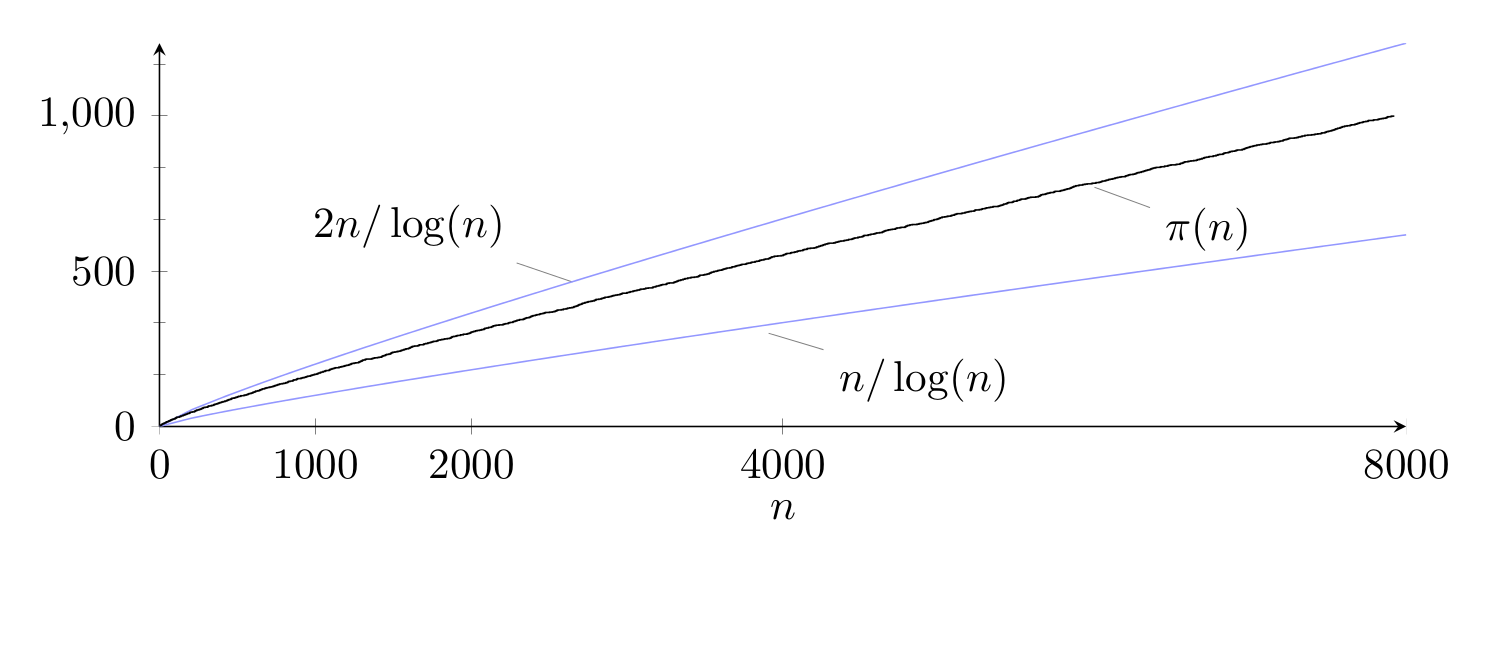
\includegraphics[scale=0.4]{img/freqPremiers.png}\end{center}\vspace{-3em}
		\caption{La fonction $\pi(n)$ pour les 1000 premiers nombres premiers}\label{fig:M3}
	\end{figure}
	
	Le tableau suivant contient l'approximation ainsi que le nombre exact de nombres premiers pour différentes valeurs de $n$. On y remarque que l'approximation est assez bonne.
	\begin{table}[H]\begin{center}
		\begin{tabular}{|lll|}
		\hline
		$n$  & $n/ln(n)$ & $\pi(n)$     \\ \hline
		$10^{3}$ & $145$     & $168$     \\
		$10^{4}$ & $1 086$   & $1 229$   \\
		$10^{5}$ & $8 686$   & $9 592$   \\
		$10^{6}$ & $72 382$  & $78 498$  \\
		$10^{7}$ & $620 420$ & $664 579$ \\ \hline
		\end{tabular}
	\end{center}\end{table}
	
	\paragraph{Probabilité de générer un nombre premier $p$ de $k$ bits :} on sait que $2^{k-1} \leqslant p \leqslant 2^{k}-1$. Le nombre de nombres premiers dans cet intervalle (c-à-d de $k$ bits) peut être approximé par :
	\[ \pi(2^{k}) - \pi(2^{k-1}) \approx \frac{2^{k}}{ln(2^{k})} - \frac{2^{k-1}}{ln(2^{k-1})} \approx \frac{2^{k-1}}{ln(2^{k-1})}	\]
	puisque $ln(2^{k}) = ln(2.2^{k-1}) = ln(2) + ln(2^{k-1})$, donc $ln(2^{k}) \approx ln(2^{k-1})$ pour $k$ grand.
	\vspace{1em}
	\\
	\noindent Donc, il y'a $2^{k-1}$ entiers $\in [2^{k-1},2^{k}-1]$ (de $k$ bits) dont approximativement $\frac{2^{k-1}}{ln(2^{k-1})}$ parmi eux qui sont premiers. Par conséquent, un nombre $p$ de $k$ bits sera premier avec une probabilité de :
	\[\frac{1}{ln(2^{k-1})}\]
	
	\paragraph{Cas de RSA-1024 :} pour générer une des deux clé de RSA-1024 dont la taille en bits est 512, on a probabilité de $1/ln(2^{511}) \approx 1/355$ pour générer un nombre premier de 512 bits. Cette chance double si on se restreint sur les entiers impairs, c'est à dire qu'on doit générer à peu près 177 nombres avant de tomber sur un nombre premier.
	
	\section{Tests de primalité}

	Les tests de primalité interviennent dans la deuxième étape du processus de génération des nombres premiers. Ce sont des algorithmes qui permettent de savoir si un nombre entier est premier. Dans le cas où le nombre n'est pas premier, il est dit \textbf{\textit{composé}}. Dans cette partie, on va détailler différents algorithmes de tests de primalité.\\
	Les tests de primalité peuvent être :
	\begin{itemize}[leftmargin=*]
		\item \textbf{déterministes :} fournissent toujours la même réponse pour un nombre donné
		\item \textbf{probabilistes :} peuvent fournir des réponses différentes pour un même nombre (utilisent des données tirées aléatoirement)
	\end{itemize}
	
	Voici la liste des différents algorithmes de tests de primalité qu'on va plus ou moins aborder :
	\begin{table}[H]\begin{center}
		\begin{tabular}{|c|c|c|}
		\hline
		Algorithme           & Année & Type       \\ \hline
		Naïf (Crible d’Eratosthène) & -240  & Déterministe \\ \hline
		Fermat               & 1640  & Probabiliste \\ \hline
		Wilson               & 1770  & Déterministe \\ \hline
		Miller-Rabin         & 1976  & Probabiliste \\ \hline
		Solovay-Strassen     & 1977  & Probabiliste \\ \hline
		AKS                  & 2002  & Déterministe \\ \hline
		\end{tabular}
	\end{center}\end{table}
	
	Certains tests seront énoncés rapidement du fait qu'il ne sont pas assez performants. Par contre, on s'intéressera plus en détail aux tests de \textit{Fermat}, \textit{Miller-Rabin}, \textit{Solovay-Strassen} et \textit{AKS}. Pour chacun de ces tests, on donnera un bref historique, son algorithme, sa complexité, sa preuve, ainsi que son implémentation.
	
		\subsection{Test naïf - Crible d’Eratosthène}
		Le test naïf représente l'idée la plus intuitive pour tester la primalité d'un nombre entier. Pour décider si un nombre $n$ est premier ou composé, on teste si les entiers $2, 3, ..., n-1$ divisent $n$. Si un parmi ces entiers divise $n$ alors on déduit que $n$ est composé, sinon on conclut qu'il est premier. Ceci revient à factoriser le nombre en question.\\
		Pour améliorer cet algorithme, on sait qu'un diviseur d'un entier $n$ quelconque ne peut dépasser $n/2$. De plus, si $n$ possède un diviseur plus grand que $\sqrt{n}$, alors il a forcement au moins un diviseur plus petit que $\sqrt{n}$. On peut donc accélérer la recherche en ne prenant en compte que des nombres premiers inférieurs à $\sqrt{n}$. Pour cela il suffit de pré-calculer et de stoker dans une table tous les nombres premiers $\leqslant \sqrt{n}$. Le \textbf{\textit{crible d'Eratosthène}} par exemple peut être utilisé dans ce but.\\
	
		\begin{algorithm}[H]
			\caption{Test naïf}\label{TN}
			\Donnees{un entier $n$}
			\Pour{tout nombre premier $p \leqslant \sqrt{n}$}{
				\Si {$p$ divise $n$}
					{\Retour composé\;}
			}
		\Retour premier\;
		\end{algorithm}
		
		\subsubsection*{Crible d'Eratosthène}
		Ce crible est un procédé établi par Eratosthène, un mathématicien grec  du III\up{e} siècle av. J.-C., qui permet de trouver tous les nombres premiers inférieurs à un certain entier naturel donné $N$. Dans notre cas, cet entier donné est $\sqrt{n}$, $n$ étant le nombre dont on va tester la primalité.\\
		L'algorithme procède par élimination : il s'agit de supprimer d'une table des entiers de $2$ à $N$ tous les multiples d'un entier. En supprimant tous les multiples, à la fin il ne restera que les entiers qui ne sont multiples d'aucun entier, et qui sont donc les nombres premiers.
		\begin{itemize}
			\item retirer les multiples du plus petit entier premier restant (multiples de 2, puis de 3, etc.)
			\item on peut s'arrêter lorsque le carré de ce plus petit entier premier restant est supérieur au plus grand entier premier restant, car dans ce cas, tous les non-premiers ont déjà été retirés précédemment
			\item à la fin du processus, tous les entiers qui n'ont pas été rayés sont les nombres premiers inférieurs à $N$
		\end{itemize}
		L'algorithme du crible est le suivant :\\ 
		
		\begin{algorithm}[H]
			\caption{Crible d'Eratosthène}\label{Eras}
			\Donnees{un entier $N$ qui correspond à $\sqrt{n}$}
			{Créer une liste L de couples \textit{(entier, primalité)}, pour les entiers allant de $2$ jusqu'à $N$, avec une primalité initialisée à "premier" : \textit{\textbf{L = \{(2, premier), (3, premier), ..., ($N$, premier)\}}} \;}
			{\textit{\textbf{plusGrandPremier}} = $N$ \;}
			\Pour{tout nombre $p$ marqué "premier" de la liste L (de manière croissante)}{
				\Si{$p^{2}$ > \textit{\textbf{plusGrandPremier}}}{ 
					\Retour L\;
				}
				{\textit{\textbf{i}} = $2$ \;}
				\Tq{$p*i < N$}{ 
					{Marquer "composé" l'entier à la position $p*i$ \;}
					{Mettre à jour \textit{\textbf{plusGrandPremier}} \;}
					{$i++$ \;}
				}
			}
		\end{algorithm}	
			
			
		\subsubsection*{Complexité}
			La complexité en temps de l'algorithme \ref{TN} (Test naïf) dans le pire des cas est de $\pi(n) \approx \frac{2\sqrt{n}}{ln(n)}$ division, c'est-à-dire $O(\sqrt{n})$ opérations. Dans le cas de RSA-1024, la complexité de cette méthode avoisine les $2^{503}$ divisions.
			
	\subsection{Test de Wilson}
	Le test de primalité de Wilson est un test déterministe basé sur le théorème suivant :
		
		\vspace{-1.5em}\begin{adjustwidth}{1.5cm}{1.5cm} 
		\begin{Th}[Théorème de Wilson]
			un entier $n > 1$ est un nombre premier si et seulement si
			\[(n-1)! + 1 \equiv 0 \pmod n\]
		\end{Th}
		\end{adjustwidth}\vspace{0.5em}
		
	Ce théorème fournit une caractérisation des nombres premiers assez anecdotique et ne constitue pas un test de primalité efficace. Son principal intérêt réside dans son histoire et dans la relative simplicité de son énoncé et de ses preuves.\\
	En effet, ce théorème était connu à partir du XVII\up{e} siècle en Europe. En 1770, \textit{John Wilson} redécouvre une conjecture de ce théorème et la publie. Ensuite, les mathématiciens \textit{Lagrange}, \textit{Euler} et \textit{Gauss} le démontrent chacun à son tour. 
		
	\subsubsection*{Algorithme}
		L'algorithme du test de primalité basé sur le théorème de Wilson est le suivant :\\
		
		\begin{algorithm}[H]
			\caption{Test de Wilson}\label{Wil}
			\Donnees{un entier $n$}
			\Si{$(n-1)! + 1 \equiv 0 \pmod n$} { 
				{\Retour premier\;}
			} \Sinon{
				{\Retour composé\;}
			}
		\end{algorithm}	
		
	\subsubsection*{Complexité}
		Ce test qui est basé sur une propriété très simple a cependant une complexité trop élevée. Il faut effectuer environ $n$ multiplications modulaires, par conséquent la complexité est de $O(n)$.

	\subsection{Test de Fermat}
	Le test de Fermat est un test de primalité probabiliste basé sur le \textit{petit théorème de Fermat} :
	
	\vspace{-1.5em}\begin{adjustwidth}{1.5cm}{1.5cm} 
	\begin{Th}[Petit théorème de Fermat (énoncé 1)]
		\label{ThFermat}
		si $p$ est un nombre premier, alors pour tout nombre entier $a$ premier avec $p$
		\[a^{p-1}\equiv 1 \pmod p\]
	\end{Th}
	\end{adjustwidth}\vspace{0.5em}
	
	Il existe un énoncé équivalent de ce théorème, qui est le suivant :
	
	\vspace{-1.5em}\begin{adjustwidth}{1.5cm}{1.5cm} 
	\begin{Th}[Petit théorème de Fermat (énoncé 2)]
		\label{ThFermat}
		si $p$ est un nombre premier, et $a$ un nombre entier quelconque, alors
		\[a^{p}\equiv a \pmod p\]
	\end{Th}
	\end{adjustwidth}\vspace{0.5em}
	
	Ce théorème doit son nom à \textit{Pierre de Fermat}, qui l'énonce la première fois en 1640. 
	
	\subsubsection{Algorithme}
		Le premier énoncé du théorème de Fermat va être exploité pour construire l'algorithme du test de primalité. Ce théorème décrit une propriété commune à tous les nombres premiers qui peut être utilisée pour détecter si un nombre est premier ou bien composé.\\
		En effet, pour $n$ est un entier dont on veut tester la primalité et $a$ un entier quelconque telle que $1 < a < n - 1$ : 
		\begin{itemize}
			\item Le fait de choisir $1 < a < n - 1$ garantit que si $n$ était premier, $a$ sera forcément premier avec $n$ (puisque $a < n - 1$) et ainsi le test n'échouera pas. 
			\item Si $\mathbf{a^{n-1} \not\equiv 1 \pmod n}$, alors $n$ est surement composé.\\
			Parmi les entiers $a$ qui ne vérifient pas l'inégalité de Fermat, il y a évidement ceux qui ne sont pas premiers avec $n$. Si l'on trouve un tel entier $a$ (qu'il soit premier ou non avec $n$), on dit que $a$ est un \textit{\textbf{témoin de non primalité}} de $n$ issu de la divisibilité.
					
					\vspace{-1.5em}\begin{adjustwidth}{1.5cm}{1.5cm} 
					\begin{Def}[Témoin de Fermat]
						\label{TemFermat}
						Soit un entier $n \geqslant 2$. On appelle témoin de Fermat pour $n$, tout entier $a$, telle que
						\[1 < a < n  \quad \text{et} \quad a^{n-1} \not\equiv 1 \pmod n\]
					\end{Def}
					\end{adjustwidth}\vspace{0.5em}
					
			\item Si $\mathbf{a^{n-1}\equiv 1 \pmod n}$, on ne peut pas conclure avec certitude que $n$ est premier puisque la réciproque du théorème de Fermat est fausse.\\
				Un nombre $n$ vérifiant cette équation peut être premier, mais aussi composé, dans ce cas $n$ est dit \textit{\textbf{pseudo-premier} de base $a$}.
					
					\vspace{-1.5em}\begin{adjustwidth}{1.5cm}{1.5cm} 
					\begin{Def}[Nombre pseudo-premier]
						\label{PseudoPrem}
						Un nombre pseudo-premier est un nombre premier probable (un entier naturel qui partage une propriété commune à tous les nombres premiers) qui n'est en fait pas premier. Un nombre pseudo-premier provenant du théorème de Fermat est appelé nombre pseudo-premier de Fermat.
					\end{Def}
					\end{adjustwidth}\vspace{0.5em}
					
				Si un nombre pseudo-premier $n$ de base $a$ est pseudo-premier pour toutes les valeurs de $a$ qui sont premières avec $n$ est appelé \textit{\textbf{nombre de Carmichael}}. 
			
					\vspace{-1.5em}\begin{adjustwidth}{1.5cm}{1.5cm} 
					\begin{Def}[Nombre de Carmichael]
						\label{Carmich}
						Un entier positif composé $n$ est appelé nombre de Carmichael si pour tout entier $a$ premier avec $n$,
						\[a^{n-1}\equiv 1 \pmod n\]
					\end{Def}
					\end{adjustwidth}\vspace{0.5em}
					
				L'entier $n = 561 = 3\ .\ 11\ .\ 17$ est le plus petit nombre de Carmichael puisque $a^{560} \equiv 1 \pmod 561$ pour tout entier $a$ premier avec $561$. Les nombres de Carmichael sont très rares. Il existe par exemple seulement $246\ 683$ nombres de Carmichael inférieurs à $10^{16}$. Le nombre de premiers inférieurs à $10^{16}$ est quant à lui égal à $279\ 238\ 341\ 033\ 925$. Donc la probabilité qu'un nombre premier inférieur à $10^{16}$ soit un nombre de Carmichael est plus petite que $1/10^{9}$.
			
		\end{itemize}
		
		\paragraph{}Les nombres pseudo-premiers et les nombre de Carmichael sont relativement rares. On peut donc envisager d'adopter ce critère pour un test probabiliste de primalité, qui est le test de Fermat. En effet, va être être répété $k$ fois, et à chaque itération, on effectue le test avec une base $a$ différente. Plus le nombre de répétitions est grand, plus la probabilité que le résultat du test soit correct augmente.\\
		
		\begin{algorithm}[H]
			\caption{Test de Fermat}\label{TF}
			\Donnees{un entier $n$ et le nombre de répétitions $k$}
			\Pour{$i$ = $1$ jusqu'à $k$}{
				Choisir aléatoirement $a$ tel que $1 < a < n - 1$\;
				\Si {$a^{p-1} \not\equiv 1 \pmod n$}
					{\Retour composé\;}
		}
		\Retour premier\;
		\end{algorithm}
		
		
	\subsubsection{Complexité}
		Si un algorithme rapide est utilisé pour l'exponentiation modulaire (par exemple Square\&Multiply), la complexité en temps de l'algorithme de Fermat est
		\[O(k\ .\ log_{2}(n)\ .\ log(log(n))\ .\ log(log(log(n))))\]
		où $k$ est le nombre de fois que le test est répété.
	
	
	\subsubsection{Preuve}
		\colorbox{yellow}{Sonny}
	\subsection{Test de Miller-Rabin}
	Le test de Miller-Rabin est un autre test de primalité probabiliste basé sur le \textit{petit théorème de Fermat} (théorème \ref{ThFermat1}). Il exploite quant à lui quelques propriétés supplémentaires. La version originale de ce test, publiée par \textit{Gary L. Miller} en 1976, est déterministe, mais ce déterminisme dépend d'une hypothèse non démontrée (hypothèse de Riemann généralisée). En 1980, \textit{Michael Rabin} a modifié cette hypothèse pour obtenir un algorithme de test probabiliste inconditionnel.
	
	\subsubsection{Algorithme}
		
		\paragraph{} Dans le cas du \textit{test de Miller-Rabin}, la propriété en question est un raffinement du \textit{petit théorème de Fermat} (théorème \ref{ThFermat1}). De la même façon que le test de Fermat, le \textit{test de Miller-Rabin} tire parti d'une propriété de l'entier $n$ dont on va tester la primalité, qui dépend d'un entier auxiliaire, le témoin $a$, et qui est vraie dès que $n$ est un nombre premier. Le principe de ce test probabiliste est donc de vérifier cette propriété pour suffisamment de témoins.
		
		\paragraph{}En effet, soit $n > 2$ un entier dont on va tester la primalité et $a$ un entier quelconque telle que $1 < a < n$. Soient $s \in \mathbb{N}^{*}$ et $t \in \mathbb{N}$ \textbf{\textit{impair}}, on peut écrire $\mathbf{n - 1 = 2^{s}t}$ ($s$ est le nombre maximum de fois que l'on peut mettre $2$ en facteur dans $n - 1$).\\
		\indent Alors, dans le cas où $n$ est premier, d'après le \textit{petit théorème de Fermat} (théorème \ref{ThFermat1}) on a :
		\begin{align*}
			a^{n-1}\equiv 1 \pmod n &\Leftrightarrow a^{2^{s}t}\equiv 1 \pmod n\\
									&\Leftrightarrow a^{2^{s}t} - 1 \equiv 0 \pmod n\\
									&\Leftrightarrow a^{2^{s}t} - 1 = (a^{2^{s-1}t})^{2} - 1 = (a^{2^{s-1}t} + 1)(a^{2^{s-1}t} - 1) \equiv 0 \pmod n	\quad	\text{(puisque } s \geqslant 1 \text{)}
		\end{align*}
		
		Si $s - 1 > 0$ alors le dernier terme est de nouveau une différence de carrés qui peut donc être factorisée. En continuant de la même manière, on obtient au final l'expression suivante :
		\[ (a^{2^{s-1}t} + 1)(a^{2^{s-2}t} + 1)...(a^{t} + 1)(a^{t} - 1) \equiv 0 \pmod n \quad\quad \text{(*)}\]
		
		On sait que pour un nombre premier $p$, si $ab \equiv 0 \pmod p$ alors $a \equiv 0 \pmod p$ ou $b \equiv 0 \pmod p$. Par conséquent, si $n$ est premier, alors l'équation (*) est vraie si et seulement si un des termes de sa partie gauche est $0 \pmod n$. Autrement dit, si $n$ est premier alors
		\[ a^{2^{j}t} \equiv -1 \pmod n \quad \text{pour au moins un } j \in \{0, 1, ..., s-1\} \]
		\[\text{ou}\]
		\[ a^{t} \equiv 1 \pmod n\]
		\indent Si pour un nombre entier $n$, une des équations ci-dessus est vérifiée, alors l'algorithme conclut que $n$ est probablement premier et termine. Si aucune de ces équations n'est vérifiée, alors l'algorithme renvoie que $n$ est composé avec certitude. On peut aussi apporter une amélioration à cette approche.\\
		\indent Si on trouve que
		\[ a^{2^{j}t} \equiv 1 \pmod n \quad \text{pour un } j \in \{0, 1, ..., s-1\} \text{,}\]
		on peut directement conclure que $n$ est composé et terminer l'exécution de l'algorithme. Ceci est dû au fait que pour un nombre $p$ premier, les seuls éléments pour lesquels un entier $x$ vérifie $x^{2} \equiv 1 \pmod p$ sont $1$ et $-1$, qui sont les deux seules racines carrées de l'unité.
		
		\paragraph{} Compte tenu de tous les éléments développés ci-dessus, l'algorithme du test de primalité de Miller-Rabin est le suivant :\\
		
		\begin{algorithm}[H]
			\caption{Test de Miller-Rabin}\label{TMR}
			\Donnees{un entier $n$ et le nombre de répétitions $k$}
			{Décomposer $n - 1 = 2^{s}t$, avec $s \in \mathbb{N}^{*}$ et $t \in \mathbb{N}$ impair \;}
			\Pour{$i$ = $1$ jusqu'à $k$}{
				{Choisir aléatoirement $a$ tel que $1 < a < n$\;}
				{$y \gets a^{t} \pmod n$\;}
				\Si{$y \not\equiv 1 \pmod n$ et $y \not\equiv -1 \pmod n$}{
					\Pour{$j = 1$ jusqu'à $s - 1$}{
						{$y \gets y^{2} \pmod n$\;}
						\Si{$y \equiv 1 \pmod n$}{
							{\Retour composé\;}
						}
						\Si{$y \equiv -1 \pmod n$}{
							{Arrêter la boucle de $j$ et continuer avec le $i$ suivant (sans renvoyer composé)\;}
						}
						{\Retour composé\;}
					}
				}
			}
			\Retour probablement premier\;
		\end{algorithm}
	
	
		\paragraph{Probabilité d'erreur et nombre d'itérations :} si le \textit{test de Miller-Rabin} renvoie composé, alors le nombre est effectivement composé. Il peut être démontré que si le test de Miller-Rabin dit que $n$ est premier, le résultat est faux avec une probabilité inférieure à $1/4$. En effet, il existe des valeurs de $a$ qui produiront de manière répétée des menteurs, qui indiqueront donc que $n$ est premier alors qu'il est composé. On appelle un \textit{\textbf{témoin}} fort pour $n$ un entier $a$ pour lequel
		\[a^{t} \not\equiv 1 \pmod n \quad \text{et} \quad a^{2^{s}j} \not\equiv -1 \pmod n \quad \text{pour tout } j \in \{0, ..., s - 1\}\]
		
		Il peut être montré qu'il existe toujours un témoin fort pour n'importe quel composé impair $n$, et qu'au moins $3/4$ de ces valeurs pour $a$ sont des témoins forts pour la composition de $n$. Si on répète ce test $k$ fois, la probabilité que le résultat soit toujours faux décroit très rapidement. La probabilité que le test renvoie premier à tort après $k$ itérations est donc de $1/4^{k}$.
		
	\subsubsection{Complexité}
		\paragraph{}Le \textit{test de Miller-Rabin} est similaire au test de Fermat. Pour prouver que nous effectuons bien de l'ordre de $log(n)$ multiplications modulaires il faut constater que nous effectuons dans Miller-Rabin $s + log_{2}(t)$ multiplications modulaires, c'est-à-dire $log_{2}(2^{s} \cdot t)$ ou bien $log_{2}(n - 1)$ car $n - 1 = 2^{s} \cdot t$
		
	\subsubsection{Preuve}
		\paragraph{}La preuve de cet algorithme repose sur la preuve du \textit{petit théorème de Fermat} de la partie précédente et des explications détaillés du principe de l'algorithme au début de cette partie.
		

	\subsection{Test de Solovay-Strassen}

	Le \textit{test de Solovay-Strassen} est un test de primalité probabiliste, publié par \textit{Robert Solovay} et \textit{Volker Strassen} en 1977. Ce test a une importance historique dans la démonstration de la faisabilité du cryptosystème RSA.

	\subsubsection{Algorithme}
		L'algorithme du \textit{test de Solovay-Strassen} est essentiellement basé sur le \textit{\textbf{critère d'Euler}}, un théorème qui énonce que :
		\vspace{-1.5em}\begin{adjustwidth}{1.5cm}{1.5cm} 
		\begin{Th}[Critère d'Euler]
			\label{CritereEuler}
			Soient $p > 2$ un nombre premier et $a$ un entier premier avec $p$
			\begin{itemize}
				\item Si $a$ est un résidu quadratique modulo $p$, alors $a^{\frac{n-1}{2}} \equiv 1 \pmod p$.
				\item Si $a$ n'est pas un résidu quadratique modulo $p$, alors $a^{\frac{n-1}{2}} \equiv -1 \pmod p$.
			\end{itemize}
			Ceci se résume en utilisant le symbole de Legendre par :
			\[a^{\frac{n-1}{2}} \equiv \left ( \frac{a}{p} \right ) \pmod p\]
		\end{Th}
		\end{adjustwidth}\vspace{0.5em}
		
		\vspace{-1.5em}\begin{adjustwidth}{1.5cm}{1.5cm} 
		\begin{Def}[Résidu quadratique]
			\label{Residu}
			On dit qu'un entier $q$ est un résidu quadratique modulo $p$ s'il existe un entier $x$ tel que :
			\[x^{2} \equiv q \pmod p\]
			Autrement dit, un résidu quadratique modulo $p$ est un nombre qui possède une racine carrée de module $p$. Dans le cas contraire, on dit que $q$ est un non-résidu quadratique modulo $p$.
		\end{Def}
		\end{adjustwidth}\vspace{0.5em}
		
		Le \textit{\textbf{symbole de Legendre}} est utilisé pour résumer le \textit{critère d'Euler}. Il est définit de la manière suivante :
		\vspace{-1.5em}\begin{adjustwidth}{1.5cm}{1.5cm} 
		\begin{Def}[Symbole de Legendre]
			\label{Legendre}
			Le symbole de Legendre est une fonction de deux variables entières à valeurs dans $\{-1, 0, 1\}$. Si $p$ est un nombre premier et $a$ un entier, alors le symbole de Legendre $\left ( \frac{a}{p} \right )$ vaut :
			\[
			\left\{
			\begin{array}{l l}
			0 & \text{si } a \text{ est divisible par } p\\
			1 & \text{si } a \text{ est un résidu quadratique modulo } p \text{ mais pas divisible par } p\\
			-1 & \text{si } a \text{ n'est pas un résidu quadratique modulo } p
			\end{array}
			\right.
			\]
			Le cas particulier $p = 2$ est inclus dans cette définition mais est sans intérêt : $\left ( \frac{a}{p} \right )$ vaut $0$ si $a$ pair et $1$ sinon.
		\end{Def}
		\end{adjustwidth}\vspace{0.5em}
		
		Pour pouvoir exploiter le \textit{critère d'Euler} dans l'algorithme du test de primalité, on doit pouvoir calculer le \textit{symbole de Legendre} pour tout entier $n$ dont on veut tester la primalité. On introduit donc le \textit{\textbf{symbole de Jacobi}} qui est une généralisation du \textit{symbole de Legendre}, définit de la manière suivante :
		\vspace{-1.5em}\begin{adjustwidth}{1.5cm}{1.5cm} 
		\begin{Def}[Symbole de Jacobi]
			\label{Jacobi}
			Le symbole de Jacobi $\left ( \frac{a}{n} \right )$ est défini, $\forall a \in \mathbb{Z}$ et $n \in \mathbb{N}$ \underline{impair}, comme produit de symboles de Legendre, en faisant intervenir la décomposition en facteurs premiers de $n$. Si $n = p_{1}*p_{2}*...*p_{k}$ pour $k \in \mathbb{N}$ telle que $p_{1}, p_{2}, ...,p_{k}$ sont des nombres premiers non nécessairement distincts, alors :
			\[\left ( \frac{a}{n} \right ) = \left ( \frac{a}{\prod_{i \in \{1,...,k\}} p_{i}} \right ) = \prod_{i \in \{1,...,k\}} \left ( \frac{a}{p_{i}} \right )\]
		\end{Def}
		\end{adjustwidth}\vspace{0.5em}
		
		Compte tenu des notions décrites ci-dessus, on peut maintenant construire l'algorithme de test de primalité de Solovay-Strassen :\\
		
		\begin{algorithm}[H]
			\caption{Test de Solovay-Strassen}\label{TSS}
			\Donnees{un entier $n$ \underline{impair} et le nombre de répétitions $k$}
			\Pour{$i$ = $1$ jusqu'à $k$}{
				Choisir aléatoirement $a$ tel que $2 < a < n$\;
				$x \gets \left ( \frac{a}{n} \right )$\;
				\Si {$x = 0$ ou $x \not\equiv a^{\frac{n-1}{2}} \pmod n$}{
					{\Retour composé\;}
				}
			}
		\Retour probablement premier\;
		\end{algorithm}
		
		\paragraph{} Cet algorithme exploite essentiellement le \textit{critère d'Euler} (théorème \ref{CritereEuler}). En effet, pour un entier $n$ dont on veut tester la primalité et un entier $a$ quelconque telle que $2 < a < n$ :
		\begin{itemize}
		\item Si $\mathbf{a^{\frac{n-1}{2}} \not\equiv \left ( \frac{a}{n} \right ) \pmod n}$, alors $n$ est surement composé.\\
		Parmi les entiers $a$ qui ne vérifient pas le \textit{critère d'Euler} (théorème \ref{CritereEuler}), il y a évidement ceux qui ne sont pas premiers avec $n$. Si l'on trouve un tel entier $a$ (qu'il soit premier ou non avec $n$), on dit que $a$ est un \textit{\textbf{témoin de non primalité}} de $n$ (\textit{témoin d'Euler}).
			
			\vspace{-1.5em}\begin{adjustwidth}{1.5cm}{1.5cm} 
			\begin{Def}[Témoin d'Euler]
			\label{TemEuler}
				Soit un entier $n > 2$. On appelle témoin d'Euler pour $n$, tout entier $a$, telle que
				\[2 < a < n  \quad \text{et} \quad a^{\frac{n-1}{2}} \not\equiv \left ( \frac{a}{n} \right ) \pmod n\]
			\end{Def}
			\end{adjustwidth}\vspace{0.5em}
		
		\item Si $\mathbf{a^{\frac{n-1}{2}} \equiv \left ( \frac{a}{n} \right ) \pmod n}$, on ne peut pas conclure avec certitude que $n$ est premier puisque la réciproque du \textit{critère d'Euler} (théorème \ref{CritereEuler}) est fausse.\\
		Un nombre $n$ vérifiant cette équation peut être premier, mais aussi composé, dans ce cas $n$ est dit \textit{\textbf{pseudo-premier d'Euler-Jacobi} de base $a$} ou menteur.
					
			\vspace{-1.5em}\begin{adjustwidth}{1.5cm}{1.5cm} 
			\begin{Def}[Nombre pseudo-premier d'Euler-Jacobi]
				\label{PseudoPremEulerJ}
				Un nombre pseudo-premier d'Euler-Jacobi de base $a$ est un nombre composé impair $n$ premier avec $a$ et tel que la congruence suivante soit vérifiée :
				\[a^{\frac{n-1}{2}} \equiv \left ( \frac{a}{n} \right ) \pmod n\]
			\end{Def}
			\end{adjustwidth}\vspace{0.5em}
			
		\indent À la différence du test de primalité de Fermat, pour chaque entier composé $n$, au moins la moitié de tous les $a$ sont des témoins d’Euler. Par conséquent, il n’y a aucune valeur de $n$ pour laquelle tous les $a$ sont des menteurs, alors que c'est le cas pour les nombres de \textit{Carmichael} dans le test de Fermat.
		\end{itemize}
	
	
	\subsubsection{Complexité}
		\paragraph{}Pour étudier la complexité du \textit{test Solovay-Strassen}, il faut étudier l'évaluation du \textit{symbole de Jacobi}. En effet, dans le corps de la boucle, à la différence du \textit{test de Fermat}, avant d'effectuer l'exponentiation modulaire nous allons évaluer un \textit{symbole de Jacobi}. La complexité d'une itération sera de l'ordre du terme dominant entre le \textit{symbole de Jacobi} et l'exponentiation modulaire.
		
		\paragraph{}Le \textit{symbole de Jacobi} $\left ( \frac{a}{b} \right )$ s'évalue en $O(log(a) \cdot log(b))$. Ainsi, dans le cadre de ce test, le \textit{symbole de Jacobi} s'évalue en $O(log(n)^{2})$.
		
		\paragraph{}L'évaluation du \textit{symbole de Jacobi} reste dominée par l'exponentiation rapide même couplée d'une multiplication modulaire rapide.\\
		\indent On rappelle qu'on avait obtenu des complexités en $O(log(n)^{2} \cdot log(log(n)) \cdot log(log(log(n))))$ en utilisant la multiplication FFT et en $ O(log(n)^{1 + log_{2}(3)})$ (avec $1 + log_{2}(3) > 2$) avec la multiplication de \textit{Karatsuba}.
				
	\subsubsection{Preuve}
		Durant cette démonstration, nous allons utiliser et admettre le \textit{théorème de Lagrange}.
		\vspace{-1.5em}\begin{adjustwidth}{1.5cm}{1.5cm} 
		\begin{Th}[Théorème de Lagrange]
			\label{ThLagrange}
			Soient $p$ un nombre premier et $f(X) \in \mathbb{Z}[X]$ un polynôme à coefficients entiers alors:
			\begin{itemize}
			\item Soit tous les coefficients de $f$ sont divisibles par $p$.
			\item Soit $f(X) \equiv 0 \text{ mod } p$ admet au plus $degre(f)$ solutions non équivalentes.
			\end{itemize}
		\end{Th}
		\end{adjustwidth}\vspace{0.5em}
		
		\paragraph{}En admettant le \textit{théorème de Lagrange}, il suffit de prouver le \textit{critère d'Euler} pour avoir une preuve satisfaisante du théorème. En effet, comme énoncé précédemment, le \textit{test de Solovay-Strassen} s'appuie directement sur la contraposée du \textit{critère d'Euler}.
		\paragraph{}Nous partirons de plusieurs constatations pour prouver le \textit{critère d'Euler} :
		\begin{enumerate}
		\item D'après le \textit{théorème de Lagrange}, comme $p$ est premier, $x^{2} \equiv a \text{ mod } p$ admet au plus deux solutions distinctes pour chaque $a$ différent. Donc, hormis $x = 0$, comme chaque racine $x$ peut être accompagnée d'une deuxième racine comme solution de l'équation, il y a au moins $(p - 1)/2$ résidus quadratiques $a$ différents. 
		\item $(\mathbb{Z}/p\mathbb{Z}, +, \cdot)$ est un corps ($p$ premier).
		\end{enumerate}
		
		\paragraph{}Pour commencer on va partir du \textit{théorème de Fermat} et le réécrire :
		\[a^{p-1} \equiv 1 \text{ mod } p \iff (a^{\frac{p-1}{2}} - 1) \cdot (a^{\frac{p-1}{2}} + 1) \equiv 0 \text{ mod } p\]
		Grâce à la constatation 2., on obtient que le produit est nul si et seulement si l'un au moins des facteurs est nul. Si $a$ est un résidu quadratique, il existe $x$ tel que $x^{2} \equiv a \text{ mod } p$, on a :
		\[
			a^{\frac{p-1}{2}} \equiv (x^{2})^{\frac{p-1}{2}} \equiv x^{p-1} \equiv 1 \text{ mod } p
		\]
		La dernière étape est obtenue à l'aide du \textit{petit théorème de Fermat}.
		
		\paragraph{}On sait que d'après le \textit{théorème de Lagrange}, $(a^{\frac{p-1}{2}} - 1) \equiv 0 \text{ mod } p$ admet au plus $(p-1)/2$ solutions pour $a$. On sait également (constatation 1.) qu'il y a au moins $(p-1)/2$ résidus quadratiques modulo $p$. Donc, il y a exactement $(p-1)/2$ valeurs qui annulent le premier facteur : les résidus quadratiques. Et, les autres $(p-1)/2$ valeurs non-résidus annulent forcément le second terme pour satisfaire le petit \textit{théorème de Fermat}.
		
		\paragraph{}\noindent En résumé :
			\begin{itemize}
				\item Si $a$ est un résidu quadratique modulo $p$, alors $a^{\frac{n-1}{2}} \equiv 1 \pmod p$.
				\item Si $a$ n'est pas un résidu quadratique modulo $p$, alors $a^{\frac{n-1}{2}} \equiv -1 \pmod p$.
			\end{itemize}

	\subsection{Test AKS}
		

	\subsubsection{Algorithme}
		\colorbox{yellow}{Younes + Idir + Sonny}
		
	\subsubsection{Complexité}
		\colorbox{yellow}{Sonny}
	
	\subsubsection{Preuve}
		\colorbox{yellow}{Sonny}
	
	\section{Mesures de performance et comparatifs}
	Dans la partie précédente, on s'est contenté de présenter différents tests de primalité sans conclue par rapport à leurs performances. Dans cette partie, on va mesurer ces performances et établir un comparatif entre les différents tests abordés.
	
	\subsection{Premiers tests déterministes}
		
		\paragraph{Algorithmes déterministes - Algorithmes probabilistes} Les tests vus dans les parties précédentes sont des exemples d'algorithmes déterministes, dont la sortie est exacte avec probabilité de 1. Leur complexité est cependant trop élevée. 
		En pratique, on utilise des algorithmes beaucoup plus efficaces pour tester la primalité d'un nombre. Il s'agit des algorithmes probabilistes. Ces algorithmes décident si un entier est premier ou pas avec une certaine probabilité $P$. La sortie d'un test de primalité probabiliste sur un entier $n$ est soit :
		\begin{itemize}
			\item $n$ est composé : toujours vrai
			\item $n$ est premier : vrai avec une probabilité $P$
		\end{itemize}
		Dans le cas où la sortie du test est "premier", il y a toujours une petite probabilité que le nombre testé ne soit pas vraiment premier. Pour pallier à ce problème et diminuer cette probabilité, on a tendance à répéter le test probabiliste un certain nombre de fois.
		
	\subsection{Tests probabilistes}
	\subsection{Tests déterministes rapides : AKS}
	\subsection{Test générique}
	

	
	
	\section{Bilan technique du projet}
		Notre produit final, c'est à dire l'application, se comporte comme prévu : l'application est fonctionnelle, la liaison entre ses différents modules réussit bien et les différentes fonctionnalités fournissent le résultat attendu.		

		\subsection{Problèmes rencontrés}
			\subsubsection*{Problèmes résolus :} 
			Lors de la réalisation de l'application, on a été confrontés à plusieurs problèmes et points délicats, principalement des verrous techniques, qui ont perturbé le bon déroulement de notre travail :
				
			\subsubsection*{Problèmes non résolus :}
				Certains problèmes rencontrés n'ont pas été entièrement résolus. Ces problèmes ne sont pas déterminants pour l'acceptabilité de notre produit.
				
		\subsection{Organisation interne du groupe}
		Assignation des modules pour chaque membre du groupe :
		Cette répartition a été parfaitement respectée. Elle nous a permis de travailler efficacement et assez indépendamment, ce qui prouve que l'assignation des modules a été judicieusement faite. Nous sommes également restés en contact pendant toute la phase de développement pour s'entraider pour la prise en main des nouveaux outils.
	
		\subsection{Coûts}
		Ce tableau indique les coûts estimés et les coûts finaux, en nombre de lignes de code et pour chaque module :
	
	\section*{Conclusion}
	
		
\end{document}
